\section{Graph Info}
This solution uses a graph to formulate constraints and describe bus availability. The graph represents a flow of chargers as they traverse a time-sequence of available buses.  By activating graph edges, we imply a certain state associated with a number of chargers. Edges leading to active layers of the graph indicate that this charger is charging a bus where an active `rest' layer gives an unused charger. The graph contains n + 1 layers, where n is the number of buses in the fleet.  There is one layer for each bus as well as a `rest' layer for non-charging elements.
\par nodes represent bus availability.  A node for bus i at time j indicates bus i's availability for charging at time j.  In Figure \ref{fig:simpleGraph2Bus}, for example, both buses one and two are available at times two, three, five, and six, and unavailable otherwise.  Note how the zeroeth element always has nodes.  This is consistent with an ever-present no-charge option.

\par Edges represent potential actions to be done between time indices and represent one of three actons: mount, charge, or dismount (see figure \ref{fig:edgeTypes}). A mount acton signals a bus to connect to a charger.  A charge action causes a bus to charge, and a dismount to disconnect. A charge command must always be lead by a mount, and followed be either an additional charge or dismount command. 
\begin{figure}
	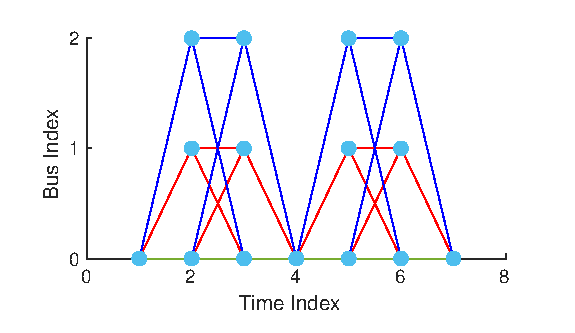
\includegraphics[width=3.5in, height=2in]{media/simpleGraph2Bus.eps}
	\caption{A simple graph with two buses and six time intervals}
	\label{fig:simpleGraph2Bus}
\end{figure}
\begin{figure}
	\centering
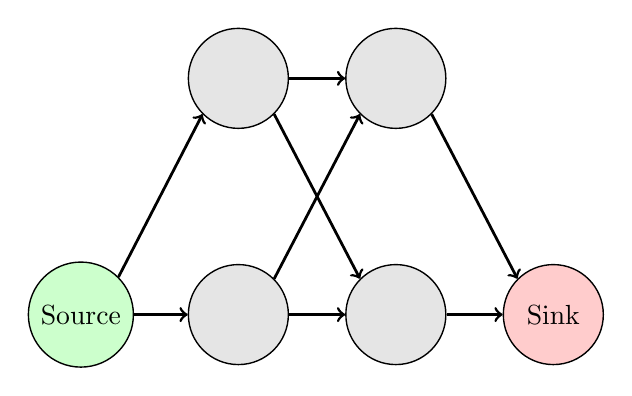
\begin{tikzpicture}
	\node[circle, fill=green!20, line width=0.5pt, draw=black, minimum size=0.5in](one) at (0,0){Source};
	\node[circle, fill=gray!20,line width=0.5pt, draw=black, minimum size=0.5in](two) at (2,0){};
	\node[circle, fill=gray!20,line width=0.5pt, draw=black, minimum size=0.5in](three) at (4,0){};
	\node[circle, fill=red!20,line width=0.5pt, draw=black, minimum size=0.5in](four) at (6,0){Sink};
	\node[circle, fill=gray!20, line width=0.5pt, draw=black, minimum size=0.5in](five) at (2,3){};
	\node[circle, fill=gray!20, line width=0.5pt, draw=black, minimum size=0.5in](six) at (4,3){};
	\draw [->, line width=1pt] (one.north east) -- (five.south west);
	\draw [->, line width=1pt] (one.east) -- (two.west);
	\draw [->, line width=1pt] (five.east) -- (six.west);
	\draw [->, line width=1pt] (five.south east) -- (three.north west);
	\draw [->, line width=1pt] (two.north east) -- (six.south west);
	\draw [->, line width=1pt] (six.south east) -- (four.north west);
	\draw [->, line width=1pt] (two.east) -- (three.west);
	\draw [->, line width=1pt] (three.east) -- (four.west); 
\end{tikzpicture}
	\caption{Network flow illustrating sources and sinks}
	\label{fig:sourceSink} 
\end{figure} 
\par This type of directed graph can be represented using an incidence matrix, where the i,jth element refers to a connection between node i and edge j.  This value is either positive or negative 1.  A positive 1 implies an incoming edge whereas negative one indicates an outgoing edge. For example, the graph given in figure \ref{fig:genericGraph} would be described as: 
\begin{figure}
	\centering
	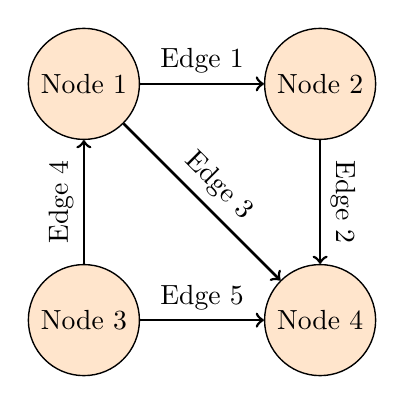
\begin{tikzpicture}
		\node[circle, line width=0.5pt, draw=black, fill=orange!20, minimum size=0.5in](topLeft) at (0,3){Node 1};
		\node[circle, line width=0.5pt, draw=black, fill=orange!20, minimum size=0.5in](topRight) at (3,3){Node 2};
		\node[circle, line width=0.5pt, draw=black, fill=orange!20, minimum size=0.5in](btmLeft) at (0,0){Node 3};
		\node[circle, line width=0.5pt, draw=black, fill=orange!20, minimum size=0.5in](btmRight) at (3,0){Node 4};
		\draw [->, line width=1pt] (topLeft.east) -- node [text width=2.5cm, midway, above, align=center]{Edge 1}(topRight.west);
		\draw [->, line width=1pt] (btmLeft.north) -- node [sloped, anchor=center, above, text width=2.5cm, midway, align=center]{Edge 4}(topLeft.south);
		\draw [->, line width=1pt] (topLeft.south east) -- node [sloped, anchor=center, above, text width=2.5cm, midway, align=center]{Edge 3}(btmRight.north west);
		\draw [->, line width=1pt] (topRight.south) -- node[sloped, anchor=center, above, text width=2.5cm, midway, align=center]{Edge 2}(btmRight.north);
		\draw [->, line width=1pt] (btmLeft.east) -- node[text width=2.5cm, midway, above, align=center]{Edge 5}(btmRight.west);
	\end{tikzpicture}
	\caption{A generic directed graph consisting of nodes and edges}
	\label{fig:genericGraph}
\end{figure}
\begin{align}
	\begin{bmatrix}
		-1 & 0 & -1 & 1 & 0 \\
		1 & -1 & 0 & 0 & 0 \\
		0 & 0 & 0 & -1 & -1 \\
		0 & 1 & 1 & 0 & 1 \\
	\end{bmatrix}
\end{align}
\par If we let $x$ be a vector representing the number of chargers occupying any one edge and $A$ be an adjacency matrix, then the total `flow' for each node can be expressed as 
\begin{align}
	\text{flow} = Ax.
\end{align}
Because chargers are not consumed or produced during the day, the total flow for each node must be zero with the exception of \textit{sources} and \textit{sinks}.  Sources are single nodes from which the first edges originate as shown in figure \ref{fig:sourceSink}, and give a negative flow value equal to the number of chargers.  A sink is converse, where the final edges terminate and maintains a corresponding positive flow value.
\begin{figure}
	\centering
	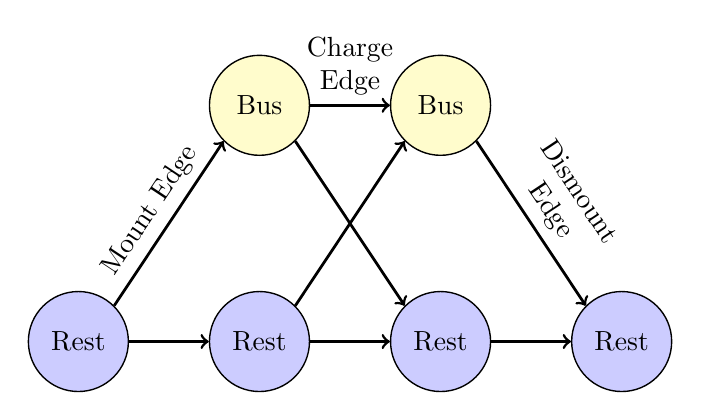
\begin{tikzpicture}
		\node[circle, fill=blue!20,line width=0.5pt, draw=black, minimum size=0.5in](one) at (0,0){Rest};
		\node[circle, fill=blue!20,line width=0.5pt, draw=black, minimum size=0.5in](two) at (2.3,0){Rest};
		\node[circle, fill=blue!20,line width=0.5pt, draw=black, minimum size=0.5in](three) at (4.6,0){Rest};
		\node[circle, fill=blue!20,line width=0.5pt, draw=black, minimum size=0.5in](four) at (6.9,0){Rest};
		\node[circle, fill=yellow!20,line width=0.5pt, draw=black, minimum size=0.5in](five) at (2.3,3){Bus};
		\node[circle, fill=yellow!20,line width=0.5pt, draw=black, minimum size=0.5in](six) at (4.6,3){Bus};
		\draw [->, line width=1pt] (one.north east) -- node[sloped, anchor=center, above, text width=2.5cm, midway, align=center]{Mount Edge}(five.south west);
		\draw [->, line width=1pt] (one.east) -- (two.west);
		\draw [->, line width=1pt] (five.east) -- node[sloped, anchor=center, above, text width=1.5cm, midway, align=center]{Charge Edge}(six.west);
		\draw [->, line width=1pt] (five.south east) -- (three.north west);
		\draw [->, line width=1pt] (two.north east) -- (six.south west);
		\draw [->, line width=1pt] (six.south east) -- node[sloped, anchor=center, above, text width=1.5cm, midway, align=center]{Dismount Edge}(four.north west);
		\draw [->, line width=1pt] (two.east) -- (three.west);
		\draw [->, line width=1pt] (three.east) -- (four.west); 
	\end{tikzpicture}
	\caption{Mount, Dismount, and Charge Edges}
	\label{fig:edgeTypes}
\end{figure}
\par This relationship can be described in terms of a \textit{flow constraint}:
\begin{align}
	Ax = \begin{bmatrix} 0 \\ \vdots \\ -\text{nCharger} \\ \vdots \\ 0 \\ \text{nCharger} \\ \vdots \\ 0\end{bmatrix}
\end{align}

\par We also assume that a bus will only charge once before departing for the next route, and that one charger can only service one bus at a time. This constraint is described as a \textit{group} constraint, where groups are collections of nodes for a single bus that describe continuous time at the hub (see figure \ref{fig:groups})
\begin{figure}
	\centering
	\begin{tikzpicture}
		\node[circle, fill=blue!20, line width=0.5pt, draw=black, minimum size=0.1in](one) at (0,0){};
		\node[circle, fill=blue!20, line width=0.5pt, draw=black, minimum size=0.1in](two) at (1,0){}; 
		\node[circle, fill=blue!20, line width=0.5pt, draw=black, minimum size=0.1in](three) at (2,0){};
		\node[circle, fill=blue!20, line width=0.5pt, draw=black, minimum size=0.1in](four) at (3,0){};
		\node[circle, fill=blue!20, line width=0.5pt, draw=black, minimum size=0.1in](five) at (4,0){};
		\node[circle, fill=blue!20, line width=0.5pt, draw=black, minimum size=0.1in](six) at (5,0){};
		\node[circle, fill=blue!20, line width=0.5pt, draw=black, minimum size=0.1in](seven) at (6,0){};
		\node[circle, fill=yellow!20, line width=0.5pt, draw=black, minimum size=0.1in](eight) at (1,2){};
		\node[circle, fill=yellow!20, line width=0.5pt, draw=black, minimum size=0.1in](nine) at (2,2){};
		\node[circle, fill=yellow!20, line width=0.5pt, draw=black, minimum size=0.1in](ten) at (4,2){}; 
		\node[circle, fill=yellow!20, line width=0.5pt, draw=black, minimum size=0.1in](eleven) at (5,2){}; 
		\node[ellipse, line width=0.5pt, draw=red, minimum height=0.4in, minimum width=1in, label=Group 1](group1) at (1.5,2){};
		\node[ellipse, line width=0.5pt, draw=red, minimum height=0.4in, minimum width=1in, label=Group 2](group2) at (4.5,2){};
		\draw [->, line width=0.5pt] (one.east) -- (two.west);
		\draw [->, line width=0.5pt] (two.east) -- (three.west);
		\draw [->, line width=0.5pt] (three.east) -- (four.west);
		\draw [->, line width=0.5pt] (four.east) -- (five.west);
		\draw [->, line width=0.5pt] (five.east) -- (six.west);
		\draw [->, line width=0.5pt] (six.east) -- (seven.west);
		\draw [->, line width=0.5pt] (one.north east) -- (eight.south west);
		\draw [->, line width=0.5pt] (two.north east) -- (nine.south west);
		\draw [->, line width=0.5pt] (four.north east) -- (ten.south west);
		\draw [->, line width=0.5pt] (five.north east) -- (eleven.south west);
		\draw [->, line width=0.5pt] (eight.south east) -- (three.north west);
		\draw [->, line width=0.5pt] (nine.south east) -- (four.north west);
		\draw [->, line width=0.5pt] (ten.south east) -- (six.north west);
		\draw [->, line width=0.5pt] (eleven.south east) -- (seven.north west);
		\draw [->, line width=0.5pt] (eight.east) -- (nine.west);
		\draw [->, line width=0.5pt] (ten.east) -- (eleven.west); 
	\end{tikzpicture}
	\caption{Example of groups in a network flow graph}
	\label{fig:groups}
\end{figure}
This behavior is described in terms of an inequality constraint
\begin{align}
	Bx \le \begin{bmatrix} 1\\ 1 \\\vdots \\ 1\end{bmatrix},
\end{align}
where $x$ is a matrix giving the number of chargers traversing an edge, and $B$ describes all mount edges (see figure \ref{fig:edgeTypes}) corresponding to the same group. In $B$, the i,jth value is one if the jth edge mounts to the ith group.  For example, the graph given in figure \ref{fig:groupEdges} would have the following group constraints:

\begin{align}
	B = \begin{bmatrix}0 & 0 & 0 & 0 & 0 & 0 & 1 & 0 & 0 & 1 & 0 & 0 & 0 & 0 & 0 & 0\\
	                   0 & 0 & 0 & 0 & 0 & 0 & 0 & 0 & 0 & 0 & 0 & 1 & 0 & 0 & 1 & 0\end{bmatrix}
\end{align}

\begin{figure}
\centering
	\begin{tikzpicture}
		\node[circle, fill=blue!20, line width=0.5pt, draw=black, minimum size=0.1in](one) at (0,0){};
		\node[circle, fill=blue!20, line width=0.5pt, draw=black, minimum size=0.1in](two) at (1,0){}; 
		\node[circle, fill=blue!20, line width=0.5pt, draw=black, minimum size=0.1in](three) at (2,0){};
		\node[circle, fill=blue!20, line width=0.5pt, draw=black, minimum size=0.1in](four) at (3,0){};
		\node[circle, fill=blue!20, line width=0.5pt, draw=black, minimum size=0.1in](five) at (4,0){};
		\node[circle, fill=blue!20, line width=0.5pt, draw=black, minimum size=0.1in](six) at (5,0){};
		\node[circle, fill=blue!20, line width=0.5pt, draw=black, minimum size=0.1in](seven) at (6,0){};
		\node[circle, fill=yellow!20, line width=0.5pt, draw=black, minimum size=0.1in](eight) at (1,2){};
		\node[circle, fill=yellow!20, line width=0.5pt, draw=black, minimum size=0.1in](nine) at (2,2){};
		\node[circle, fill=yellow!20, line width=0.5pt, draw=black, minimum size=0.1in](ten) at (4,2){}; 
		\node[circle, fill=yellow!20, line width=0.5pt, draw=black, minimum size=0.1in](eleven) at (5,2){}; 
		\node[ellipse, line width=0pt, draw=white, minimum height=0.4in, minimum width=1in, label=Group 1](group1) at (1.5,2){};
		\node[ellipse, line width=0pt, draw=white, minimum height=0.4in, minimum width=1in, label=Group 2](group2) at (4.5,2){};
		\draw [->, line width=0.5pt,color=black!40] (one.east) -- (two.west);
		\draw [->, line width=0.5pt,color=black!40] (two.east) -- (three.west);
		\draw [->, line width=0.5pt,color=black!40] (three.east) -- (four.west);
		\draw [->, line width=0.5pt,color=black!40] (four.east) -- (five.west);
		\draw [->, line width=0.5pt,color=black!40] (five.east) -- (six.west);
		\draw [->, line width=0.5pt,color=black!40] (six.east) -- (seven.west);
		\draw [->, color=red, line width=0.75pt] (one.north east) -- node[sloped, anchor=center, above, text width=2.5cm, align=center]{Edge 7}(eight.south west);
		\draw [->, color=red, line width=0.75pt] (two.north east) -- node[sloped, anchor=center, above, text width=2.5cm, align=center]{Edge 10}(nine.south west);
		\draw [->, color=red, line width=0.75pt] (four.north east) -- node[sloped, anchor=center, above, text width=2.5cm, align=center]{Edge 12}(ten.south west);
		\draw [->, color=red, line width=0.75pt] (five.north east) -- node[sloped, anchor=center, above, text width=2.5cm, align=center]{Edge 15}(eleven.south west);
		\draw [->, line width=0.5pt,color=black!40] (eight.south east) -- (three.north west);
		\draw [->, line width=0.5pt,color=black!40] (nine.south east) -- (four.north west);
		\draw [->, line width=0.5pt,color=black!40] (ten.south east) -- (six.north west);
		\draw [->, line width=0.5pt,color=black!40] (eleven.south east) -- (seven.north west);
		\draw [->, line width=0.5pt,color=black!40] (eight.east) -- (nine.west);
		\draw [->, line width=0.5pt,color=black!40] (ten.east) -- (eleven.west); 
	\end{tikzpicture}
	\caption{Mount edge example for groups}
	\label{fig:groupEdges}

\end{figure} 
\section{Multi-Graph Additions}
An additional contribution this work offers is the expansion to night vs day charging. During the night, there is one charger for each bus; each with a single charge rate.  During this time, buses are also available to charge at any time.  These differences in operations introduce changes to the original graph formation and warrent a separate graph.  
\par Night graphs consider a situation where both the number of buses reflecte the number of chargers and buses are readily available.  Note how there are several source and sink nodes in figure \ref{fig:nightVsDayGraph}.  When a bus deploys for the day, the available number of charges changes and are reflected in the underlying source and sink constraints.
\begin{figure*}
	\centering
	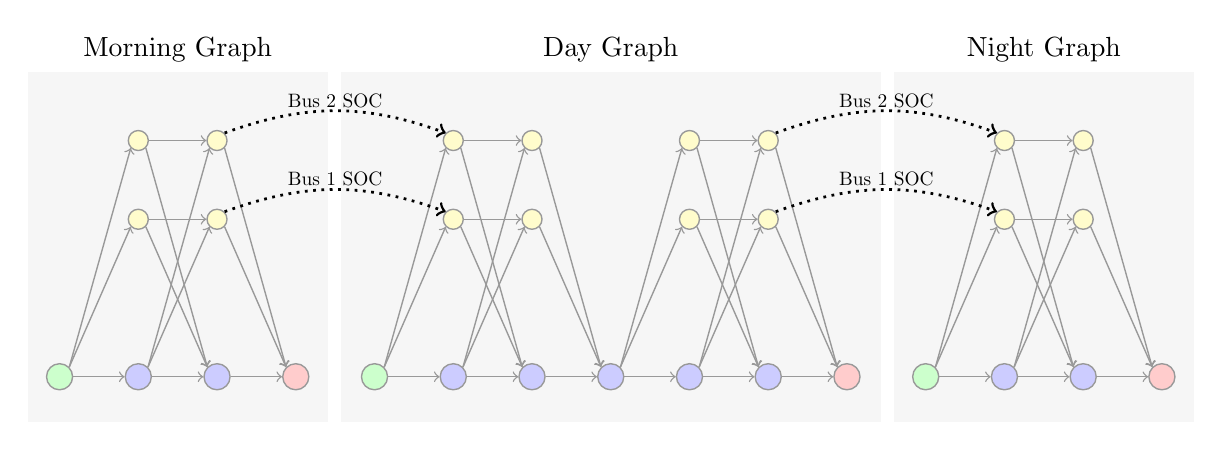
\begin{tikzpicture} 
		% morning graph
		\node[rectangle, fill=gray!7, minimum width=1.5in, minimum height=1.75in, label=above:Morning Graph](mBox) at (-2.5,1.65){};
		\node[circle, fill=green!20, line width=0.5pt, draw=black!40, minimum size=0.1in](mOne) at (-4,0){};
		\node[circle, fill=blue!20, line width=0.5pt, draw=black!40, minimum size=0.1in](mTwo) at (-3,0){}; 
		\node[circle, fill=blue!20, line width=0.5pt, draw=black!40, minimum size=0.1in](mThree) at (-2,0){};
		\node[circle, fill=red!20, line width=0.5pt, draw=black!40, minimum size=0.1in](mFour) at (-1,0){};

		\node[circle, fill=yellow!20, line width=0.5pt, draw=black!40, minimum size=0.1in, inner sep=1pt](mFive) at (-3,2){};
		\node[circle, fill=yellow!20, line width=0.5pt, draw=black!40, minimum size=0.1in, inner sep=1pt](mSix) at (-2,2){};
		\node[circle, fill=yellow!20, line width=0.5pt, draw=black!40, minimum size=0.1in, inner sep=1pt](mSeven) at (-3,3){};
		\node[circle, fill=yellow!20, line width=0.5pt, draw=black!40, minimum size=0.1in, inner sep=1pt](mEight) at (-2,3){};

		\draw[->, line width=0.5pt, color=black!40] (mOne.east) -- (mTwo.west){};
		\draw[->, line width=0.5pt, color=black!40] (mTwo.east) -- (mThree.west){};
		\draw[->, line width=0.5pt, color=black!40] (mThree.east) -- (mFour.west){};

		\draw[->, line width=0.5pt, color=black!40] (mOne.north east) -- (mFive.south west){};
		\draw[->, line width=0.5pt, color=black!40] (mTwo.north east) -- (mSix.south west){};
		\draw[->, line width=0.5pt, color=black!40] (mOne.north east) -- (mSeven.south west){};
                \draw[->, line width=0.5pt, color=black!40] (mTwo.north east) -- (mEight.south west){};

                \draw[->, line width=0.5pt, color=black!40] (mFive.south east) -- (mThree.north west){}; 
                \draw[->, line width=0.5pt, color=black!40] (mSix.south east) -- (mFour.north west){};
                \draw[->, line width=0.5pt, color=black!40] (mSeven.south east) -- (mThree.north west){};
		\draw[->, line width=0.5pt, color=black!40] (mEight.south east) -- (mFour.north west){};

                \draw[->, line width=0.5pt, color=black!40] (mFive.east) -- (mSix.west){};
                \draw[->, line width=0.5pt, color=black!40] (mSeven.east) -- (mEight.west){};

		% night graph
		\node[rectangle, fill=gray!7, minimum width=1.5in, minimum height=1.75in, label=above:Night Graph](nBox) at (8.5,1.65){};
		\node[circle, fill=green!20, line width=0.5pt, draw=black!40, minimum size=0.1in](nOne) at (7,0){};
		\node[circle, fill=blue!20, line width=0.5pt, draw=black!40, minimum size=0.1in](nTwo) at (8,0){}; 
		\node[circle, fill=blue!20, line width=0.5pt, draw=black!40, minimum size=0.1in](nThree) at (9,0){};
		\node[circle, fill=red!20, line width=0.5pt, draw=black!40, minimum size=0.1in](nFour) at (10,0){};

		\node[circle, fill=yellow!20, line width=0.5pt, draw=black!40, minimum size=0.1in, inner sep=1pt](nFive) at (8,2){};
		\node[circle, fill=yellow!20, line width=0.5pt, draw=black!40, minimum size=0.1in, inner sep=1pt](nSix) at (9,2){};
		\node[circle, fill=yellow!20, line width=0.5pt, draw=black!40, minimum size=0.1in, inner sep=1pt](nSeven) at (8,3){};
		\node[circle, fill=yellow!20, line width=0.5pt, draw=black!40, minimum size=0.1in, inner sep=1pt](nEight) at (9,3){};

		\draw[->, line width=0.5pt, color=black!40] (nOne.east) -- (nTwo.west){};
		\draw[->, line width=0.5pt, color=black!40] (nTwo.east) -- (nThree.west){};
		\draw[->, line width=0.5pt, color=black!40] (nThree.east) -- (nFour.west){};

		\draw[->, line width=0.5pt, color=black!40] (nOne.north east) -- (nFive.south west){};
		\draw[->, line width=0.5pt, color=black!40] (nTwo.north east) -- (nSix.south west){};
		\draw[->, line width=0.5pt, color=black!40] (nOne.north east) -- (nSeven.south west){};
                \draw[->, line width=0.5pt, color=black!40] (nTwo.north east) -- (nEight.south west){};

                \draw[->, line width=0.5pt, color=black!40] (nFive.south east) -- (nThree.north west){}; 
                \draw[->, line width=0.5pt, color=black!40] (nSix.south east) -- (nFour.north west){};
		\draw[->, line width=0.5pt, color=black!40] (nSeven.south east) -- (nThree.north west){};
		\draw[->, line width=0.5pt, color=black!40] (nEight.south east) -- (nFour.north west){};

		\draw[->, line width=0.5pt, color=black!40] (nFive.east) -- (nSix.west){};
                \draw[->, line width=0.5pt, color=black!40] (nSeven.east) -- (nEight.west){};


		% day graph	
		\node[rectangle, fill=gray!7, minimum width=2.7in, minimum height=1.75in, label=above:Day Graph](dBox) at (3,1.65){}; 
		\node[circle, fill=green!20, line width=0.5pt, draw=black!40, minimum size=0.1in](one) at (0,0){};
		\node[circle, fill=blue!20, line width=0.5pt, draw=black!40, minimum size=0.1in](two) at (1,0){}; 
		\node[circle, fill=blue!20, line width=0.5pt, draw=black!40, minimum size=0.1in](three) at (2,0){};
		\node[circle, fill=blue!20, line width=0.5pt, draw=black!40, minimum size=0.1in](four) at (3,0){};
		\node[circle, fill=blue!20, line width=0.5pt, draw=black!40, minimum size=0.1in](five) at (4,0){};
		\node[circle, fill=blue!20, line width=0.5pt, draw=black!40, minimum size=0.1in](six) at (5,0){};
		\node[circle, fill=red!20, line width=0.5pt, draw=black!40, minimum size=0.1in](seven) at (6,0){};
		
		\node[circle, fill=yellow!20, line width=0.5pt, draw=black!40, minimum size=0.1in, inner sep=1pt](eight) at (1,2){};
		\node[circle, fill=yellow!20, line width=0.5pt, draw=black!40, minimum size=0.1in, inner sep=1pt](nine) at (2,2){};
		\node[circle, fill=yellow!20, line width=0.5pt, draw=black!40, minimum size=0.1in, inner sep=1pt](ten) at (4,2){};
		\node[circle, fill=yellow!20, line width=0.5pt, draw=black!40, minimum size=0.1in, inner sep=1pt](eleven) at (5,2){};

		\node[circle, fill=yellow!20, line width=0.5pt, draw=black!40, minimum size=0.1in, inner sep=1pt](twelve) at (1,3){};
		\node[circle, fill=yellow!20, line width=0.5pt, draw=black!40, minimum size=0.1in, inner sep=1pt](thirteen) at (2,3){};
		\node[circle, fill=yellow!20, line width=0.5pt, draw=black!40, minimum size=0.1in, inner sep=1pt](fourteen) at (4,3){};
		\node[circle, fill=yellow!20, line width=0.5pt, draw=black!40, minimum size=0.1in, inner sep=1pt](fifteen) at (5,3){};

		\draw [->, line width=0.5pt, color=black!40] (one.east) -- (two.west);
		\draw [->, line width=0.5pt, color=black!40] (two.east) -- (three.west);
		\draw [->, line width=0.5pt, color=black!40] (three.east) -- (four.west);
		\draw [->, line width=0.5pt, color=black!40] (four.east) -- (five.west);
		\draw [->, line width=0.5pt, color=black!40] (five.east) -- (six.west);
		\draw [->, line width=0.5pt, color=black!40] (six.east) -- (seven.west);

		\draw [->, line width=0.5pt, color=black!40] (one.north east) -- (eight.south west);
		\draw [->, line width=0.5pt, color=black!40] (two.north east) -- (nine.south west);
		\draw [->, line width=0.5pt, color=black!40] (four.north east) -- (ten.south west);
		\draw [->, line width=0.5pt, color=black!40] (five.north east) -- (eleven.south west);
		\draw [->, line width=0.5pt, color=black!40] (eight.south east) -- (three.north west);
		\draw [->, line width=0.5pt, color=black!40] (nine.south east) -- (four.north west);
		\draw [->, line width=0.5pt, color=black!40] (ten.south east) -- (six.north west);
		\draw [->, line width=0.5pt, color=black!40] (eleven.south east) -- (seven.north west);
		\draw [->, line width=0.5pt, color=black!40] (eight.east) -- (nine.west);
		\draw [->, line width=0.5pt, color=black!40] (ten.east) -- (eleven.west); 

		\draw [->, line width=0.5pt, color=black!40] (one.north east) -- (twelve.south west);
		\draw [->, line width=0.5pt, color=black!40] (two.north east) -- (thirteen.south west);
		\draw [->, line width=0.5pt, color=black!40] (four.north east) -- (fourteen.south west);
		\draw [->, line width=0.5pt, color=black!40] (five.north east) -- (fifteen.south west);
		\draw [->, line width=0.5pt, color=black!40] (twelve.south east) -- (three.north west);
		\draw [->, line width=0.5pt, color=black!40] (thirteen.south east) -- (four.north west);
		\draw [->, line width=0.5pt, color=black!40] (fourteen.south east) -- (six.north west);
		\draw [->, line width=0.5pt, color=black!40] (fifteen.south east) -- (seven.north west);
		\draw [->, line width=0.5pt, color=black!40] (twelve.east) -- (thirteen.west);
		\draw [->, line width=0.5pt, color=black!40] (fourteen.east) -- (fifteen.west); 


		\draw [dotted, color=black,-,line width=1pt] (mSix.north east) edge[->,bend left=20pt]node[above=-2.5pt]{\scalebox{0.7}{Bus 1 SOC}}(eight.north west); 
		\draw [dotted, color=black,-,line width=1pt] (mEight.north east) edge[->,bend left=20pt]node[above=-2.5pt]{\scalebox{0.7}{Bus 2 SOC}}(twelve.north west);

		\draw [dotted, color=black,-,line width=1pt] (eleven.north east) edge[->,bend left=20pt]node[above=-2.5pt]{\scalebox{0.7}{Bus 1 SOC}}(nFive.north west); 
		\draw [dotted, color=black,-,line width=1pt] (fifteen.north east) edge[->,bend left=20pt]node[above=-2.5pt]{\scalebox{0.7}{Bus 2 SOC}}(nSeven.north west);
	\end{tikzpicture}
	\caption{Night vs Day Graphs}
	\label{fig:nightVsDayGraph}
\end{figure*}
\par Changes in the first graph are reflected in the second through use of state of charge variables.
